\documentclass[a4paper,10pt]{article}

% ---------- Packages ----------
\usepackage[a4paper,margin=1.5cm]{geometry}
\usepackage{paracol}          % two columns
\usepackage{tikz}             % graphics (photo circle + bars)
\usepackage{xcolor}
\usepackage{graphicx}
\usepackage{enumitem}
\usepackage[hidelinks]{hyperref}
\usepackage{fontawesome}      % reliable icons for pdfLaTeX (v4 set)
\usepackage{titlesec}

% ---------- Colors ----------
\definecolor{maincolor}{HTML}{D23F31}
\definecolor{textgray}{gray}{0.20}
\definecolor{barbg}{gray}{0.90}

% ---------- Spacing tweaks ----------
\setlength{\columnsep}{1.0cm}
\setlist[itemize]{noitemsep, topsep=1pt, leftmargin=1.2em}
\setlength{\parskip}{4pt}
\setlength{\parindent}{0pt}

% ---------- Language bar (0–5) ----------
\newcommand{\langbar}[1]{%
  \begin{tikzpicture}[baseline=-0.6ex]
    \fill[barbg]   (0,0) rectangle (5cm, 1.6pt);
    \pgfmathsetmacro{\w}{min(max(#1,0),5)*1.0} % clamp 0..5
    \fill[maincolor] (0,0) rectangle (\w cm, 1.6pt);
  \end{tikzpicture}%
}

% ---------- Section title ----------
\newcommand{\sect}[1]{\vspace{9pt}\textbf{\large #1}\vspace{-10pt}\par\textcolor{maincolor}{\rule{\linewidth}{0.8pt}}\vspace{4pt}}

\begin{document}\pagestyle{empty}\color{textgray}

% Control column widths (left:right)
\columnratio{0.36}
\begin{paracol}{2}

% ================= LEFT COLUMN =================
\begin{center}
  % Photo placeholder (circle)
  \begin{tikzpicture}
    %\draw[fill=barbg, draw=none] (0,0) circle (2.1cm);
    % Add your photo by replacing the fill with:
    \clip (0,0) circle (2.1cm);
    \node at (0,0) {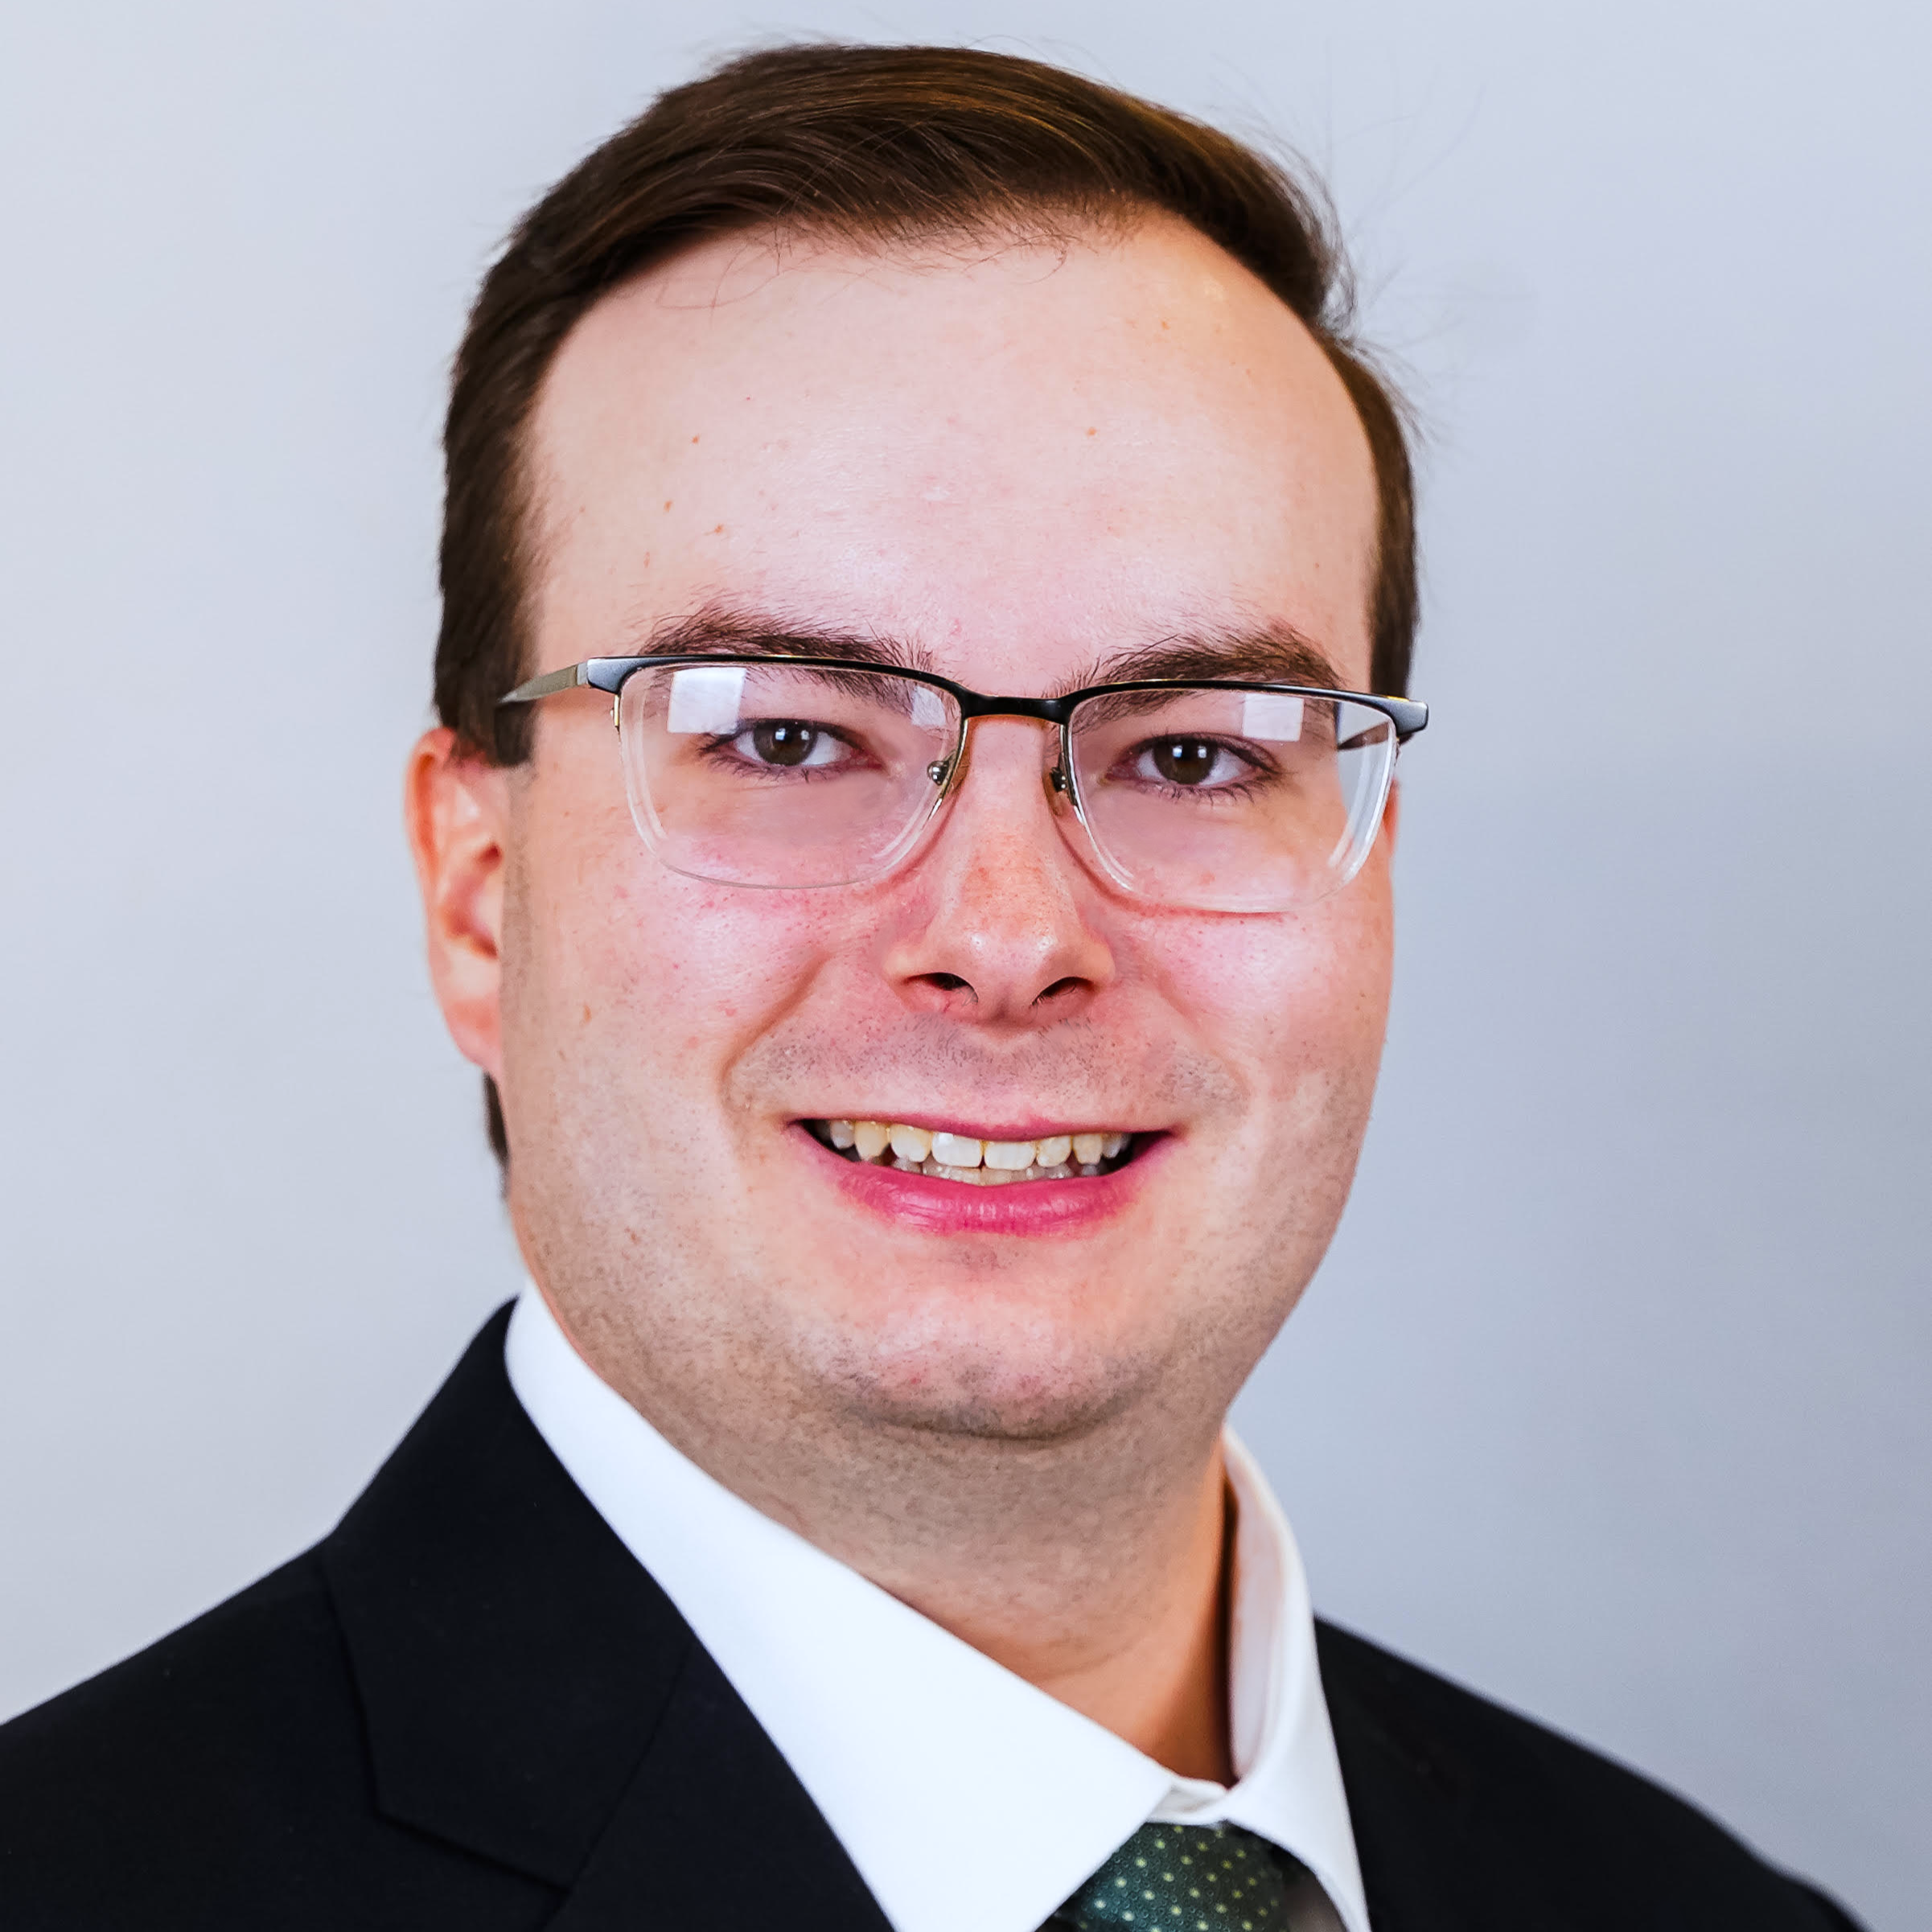
\includegraphics[width=4.2cm]{ColumHeadshot2_square.png}};
  \end{tikzpicture}

  \vspace{6pt}
  {\LARGE \textbf{Colum Cross}}\\[2pt]
  \textcolor{maincolor}{\rule{3.5cm}{1pt}}
\end{center}

\vspace{6pt}
\sect{Kontakt}
{\faPhone} ~ +1 (518) 956-3953\\
{\faPhone} ~ +49 162 8193963\\
{\faMapMarker} ~ Fischerinsel 15, 10179 Berlin\\
{\faEnvelopeO} ~ \href{mailto:columcross@gmail.com}{columcross@gmail.com}\\
{\faGlobe} ~ \href{https://columcross.com}{columcross.com}\\
{\faLinkedin} ~ \href{https://www.linkedin.com/in/columcross/}{linkedin.com/in/columcross}\\
{\faGithub} ~ \href{https://github.com/columcross}{github.com/columcross}\par

\sect{Sprachen}
\textbf{Englisch} — Muttersprache\\
\textbf{Deutsch} — Konversationssicher\par
\textbf{Programmiersprachen}
\begin{itemize}
    \item ServiceNow Developer: CSM, FSO, ITSM, SPM, Virtual Agent
    \item \textit{Frontend:} JS, Angular, React
    \item \textit{Backend:} Java, ColdFusion, PHP, Python
    \item \textit{Database:} MySQL, T-SQL, Oracle
    \item \textit{Mobile:} Java, Swift, C\#
\end{itemize}

\sect{Fähigkeiten}
\begin{itemize}
    \item ServiceNow-Plattformentwicklung
    \item Frontend- und Backend-Entwickler
    \item Beherrschung der Agile- und Scrum-Methoden
    \item Erfahrung in Endbenutzertests und\\ Usability-Forschung
\end{itemize}

\sect{Anlagen}
\begin{itemize}
    \item ServiceNow Certified Application Developer
    \item ServiceNow Certified System Administrator
    \item Certified Lean Practitioner
\end{itemize}

\sect{Hobbys}
\begin{itemize}
    \item Reisen
    \item Schreibmaschinen- und Uhrensammeln
    \item Modelleisenbahn
\end{itemize}

\switchcolumn

% ================= RIGHT COLUMN =================

\sect{Berufserfahrung}

% === M&T ===
\textbf{Software Engineer II} \hfill M\&T Bank\\
2019 - 2025 \hfill \textit{Buffalo, New York}\par
\begin{itemize}
    \item Anforderungsanalyse und Priorisierung mit Stakeholdern und Product Ownern  
    \item Konzeption und Umsetzung von ServiceNow-Oberflächen  
    \item Durchführung von Usability-Tests  
    \item Entwicklung zentraler ServiceNow-Funktionalitäten  
    \item Design und Implementierung von APIs und Integrationen  
    \item Steuerung von Codebereitstellungen in Produktion  
    \item Migration vom Update-Set- zum Application-Publishing-Modell  
    \item Leitung eines Projekts zur Mitarbeiterbindung für eine Großbank (200 Mrd. USD)  
    \item Ehrenamtliche Förderung digitaler Kompetenzen von Kindern  
    \item Durchführung technischer und verhaltensbezogener Interviews
\end{itemize}
\medskip

% === RIT ===
\textbf{Web Developer} \hfill RIT Admissions\\
2018 \hfill \textit{Rochester, New York}\par
\begin{itemize}
    \item Entwicklung von Frontend-Lösungen für interne und externe Webanwendungen  
    \item Design und Umsetzung eines interaktiven Kiosks für den Eingangsbereich der Zulassungsabteilung  
\end{itemize}
\medskip

% === Ahold ===
\textbf{Web Developer} \hfill Ahold USA\\
2017 \hfill \textit{Quincy, Massachusetts}\par
\begin{itemize}
    \item Entwicklung einer ColdFusion-API für eine Angular-Anwendung zur lokalen Produktbestellung  
    \item Umsetzung einer Angular-App und ColdFusion-API zur zentralen E-Mail-Verwaltung  
    \item Modernisierung eines Java-Backends in ColdFusion zur Verarbeitung großer Datenmengen  
\end{itemize}

% === SEFCU ===
\textbf{Web Intern} \hfill State Employees Federal Credit Union\\
2016 \hfill \textit{Albany, New York}\par
\begin{itemize}
    \item Entwicklung einer ColdFusion-Anwendung zur Generierung von News-lettern für das Unternehmen
\end{itemize}

% ============

\sect{Ausbildung}
\textbf{Rochester Institute of Technology}
\\ BS in Human-Centered Computing\par

\sect{Persönliche Projekte}
\textbf{Permission Granted} \hfill \textit{Java for Android}\\	
Eine App für Videofilmer, Vlogger und alle, die regelmäßig Freigabeformulare verwenden. Benutzer können Freigabeformulare schnell und einfach direkt auf ihrem Telefon erstellen, anzeigen und unterzeichnen.\par
\textbf{Warmer Colder} \hfill \textit{Java for Android}\\	
Ein Spiel für zwei Spieler, das auf Ihrem Standort basiert. Verwendet die Android Location API, um die Nähe zu einem Standort zu bestimmen.\par
\textbf{Tip Calculator for WearOS} \hfill \textit{Java for Android}\\
Eine Anwendung ausschließlich für Wear OS-Geräte. Sie berechnet ein Trinkgeld und den Gesamtbetrag basierend auf einem Grundpreis und einem Trinkgeldprozentsatz.\par
\textbf{Math Based N-Back Test} \hfill \textit{C\# Universal Windows App}\\
Eine Anwendung, die das Arbeitsgedächtnis testet, indem den Teilnehmern eine Reihe einstelliger Mathefragen angezeigt werden und sie dann die Antwort auf die vorherige Frage geben müssen.


\end{paracol}
\end{document}